\chapter{\ifproject%
\ifcpe การทดลองและผลลัพธ์\else Experimentation and Results\fi
\else%
\ifcpe การประเมินระบบ\else System Evaluation\fi
\fi}


\begin{figure}
    \begin{center}
      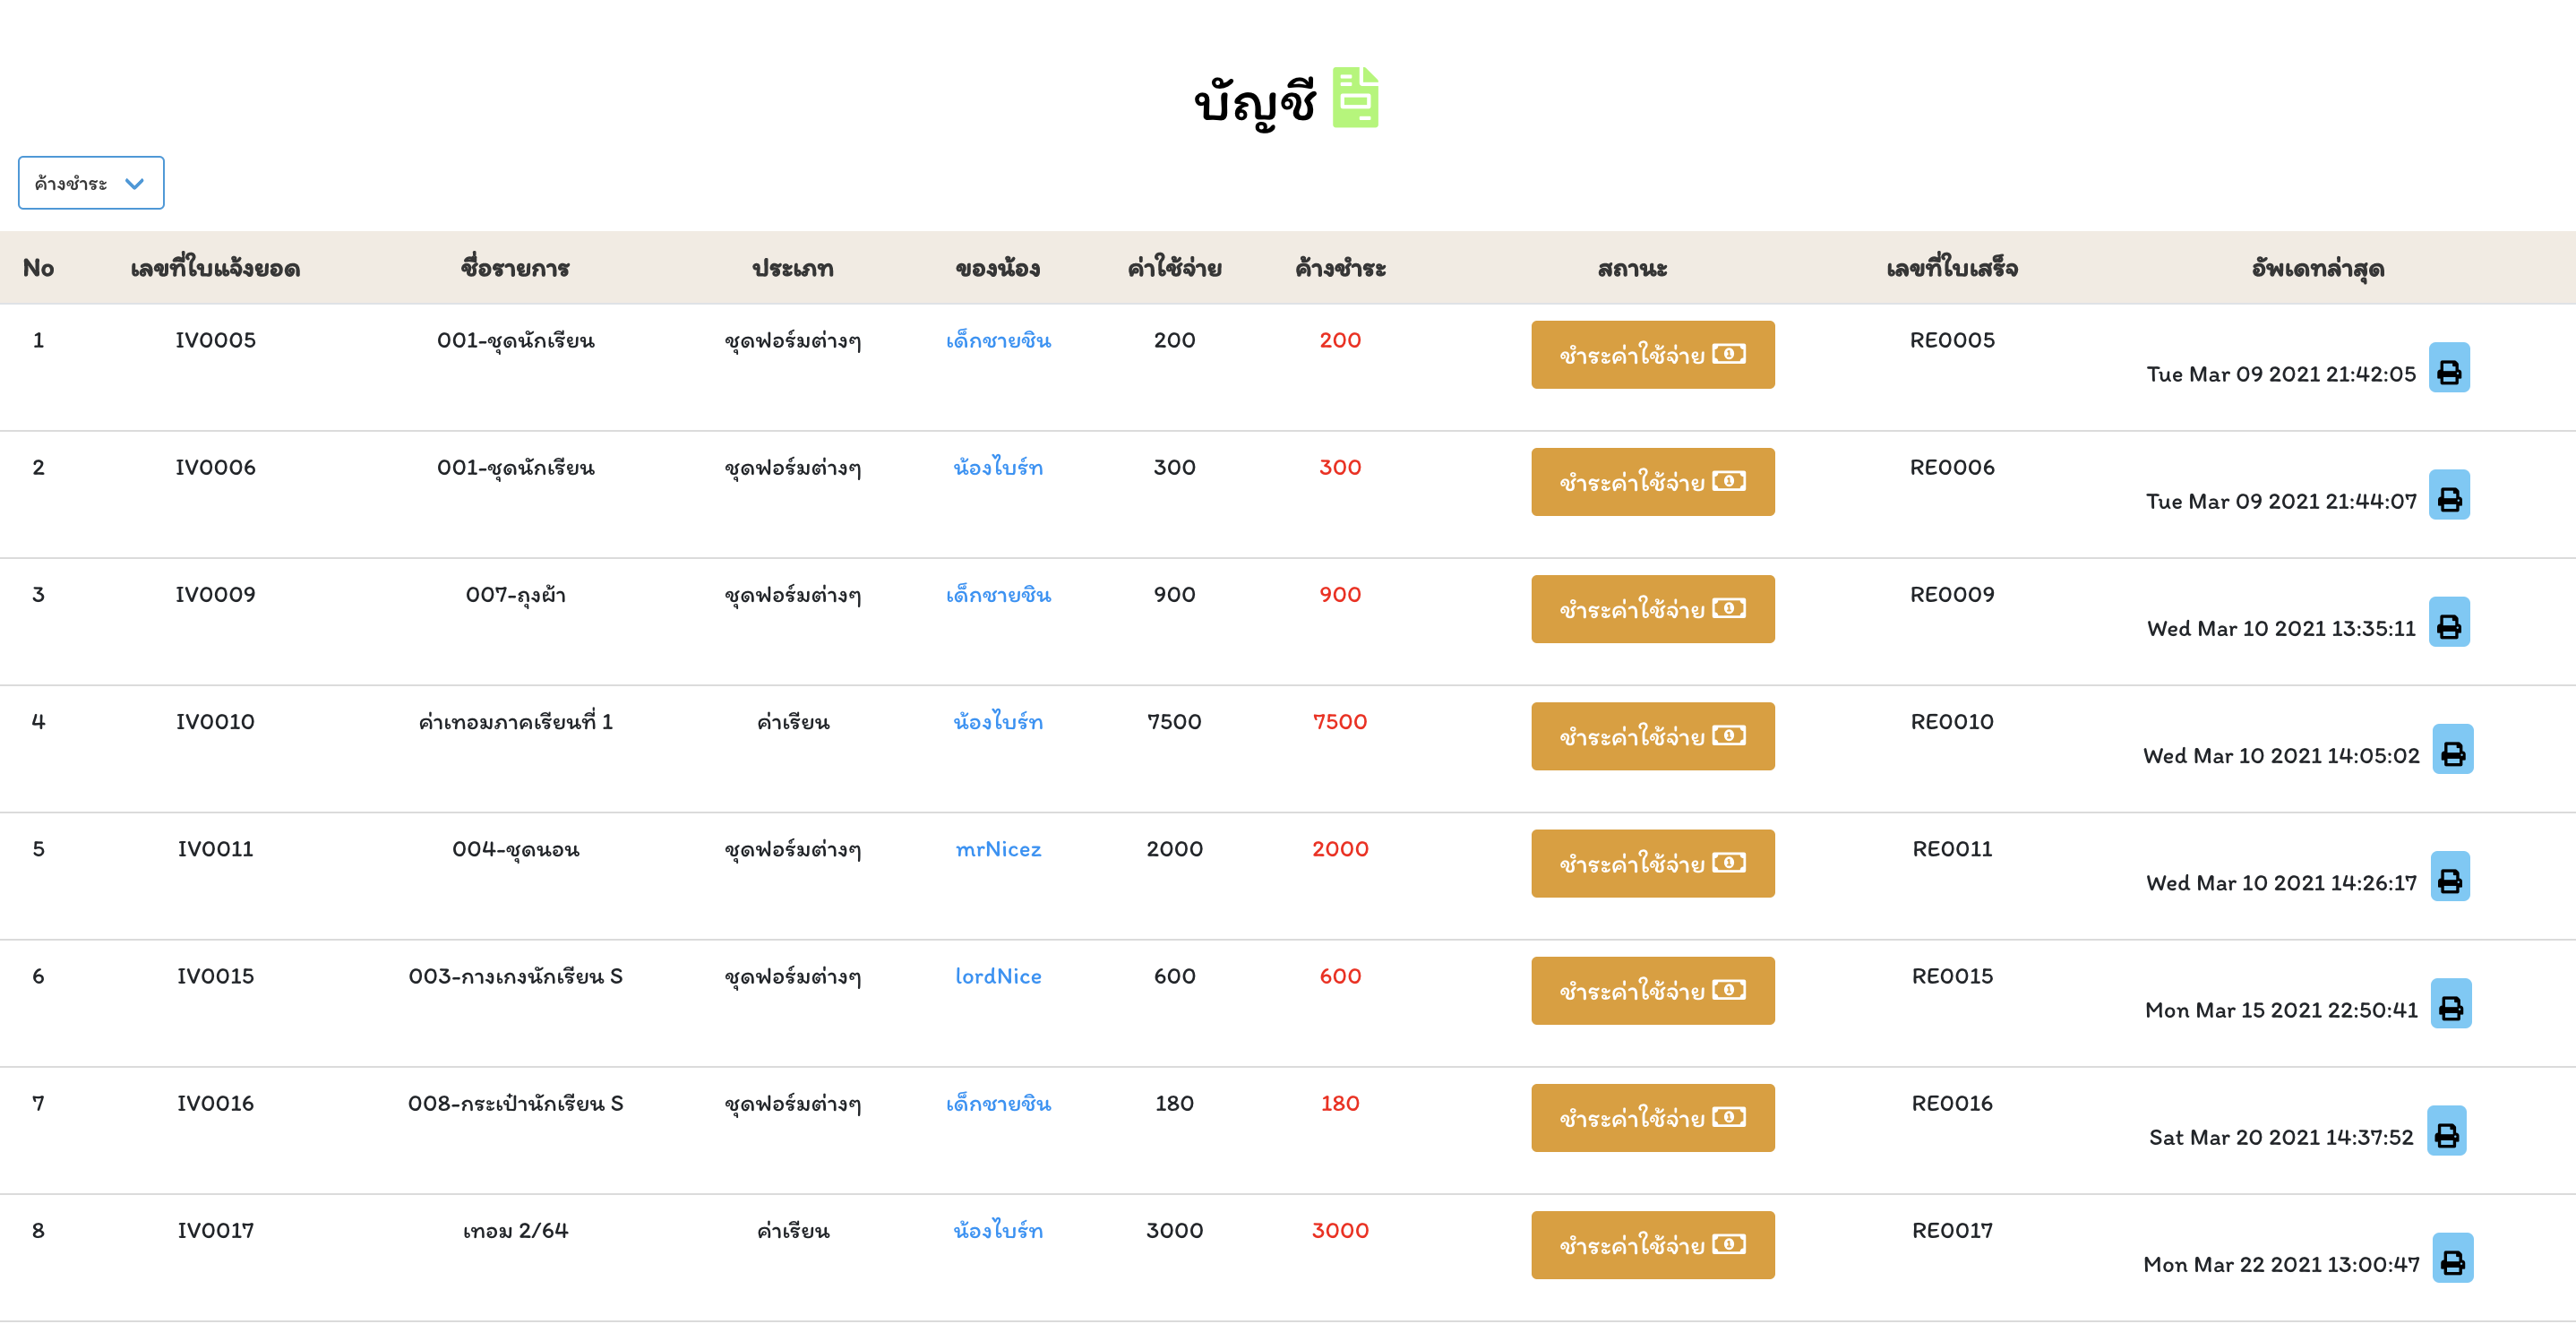
\includegraphics[width=\linewidth]{images/Payment.png}
    \end{center}
    \caption[Poem]{หน้าระบบบัญชีใหม่}
    \label{fig:PaymentNew}
\end{figure}

\begin{figure}
    \begin{center}
      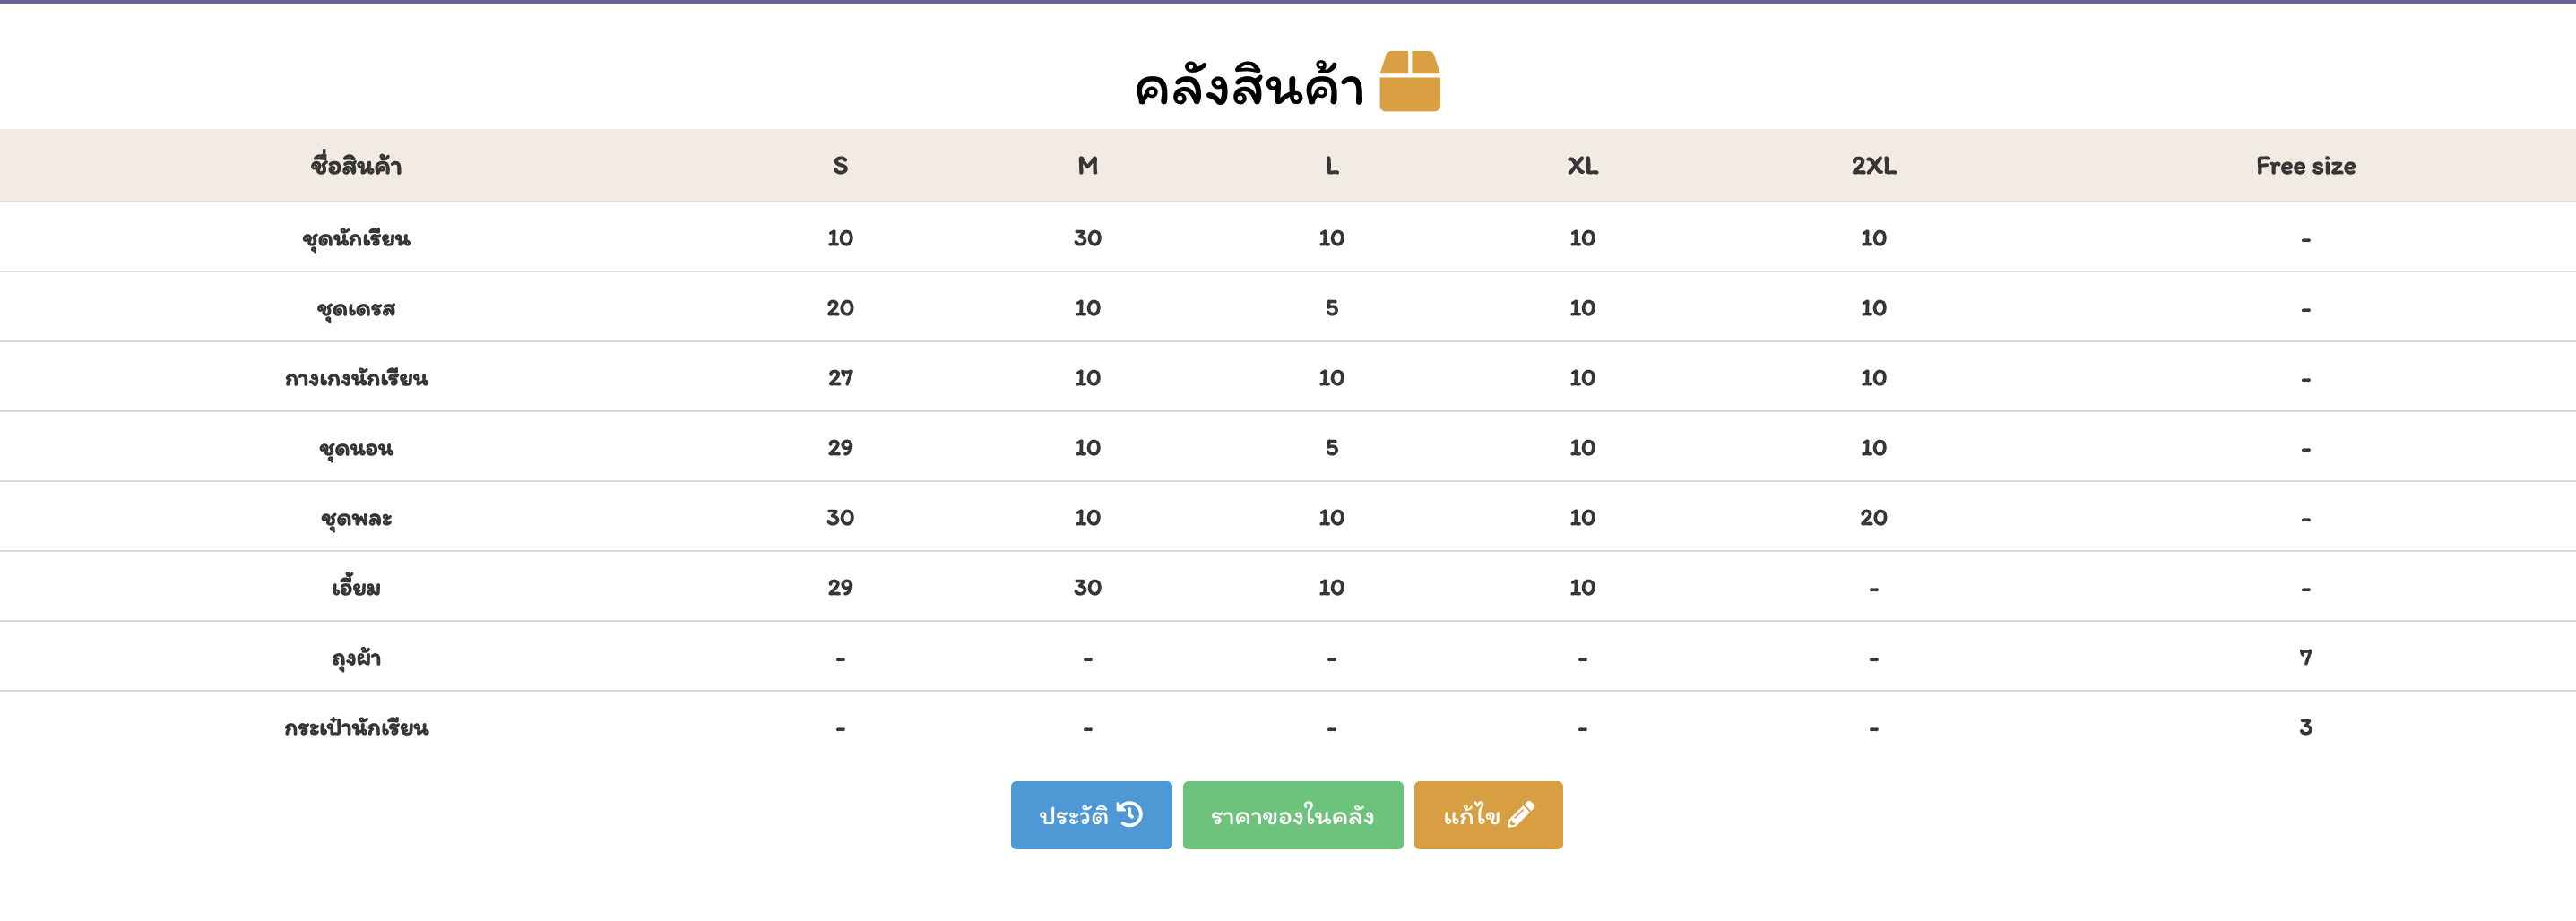
\includegraphics[width=\linewidth]{images/Stock.png}
    \end{center}
    \caption[Poem]{หน้าระบบคลักสินค้าใหม่}
    \label{fig:StockNew}
\end{figure}

\begin{figure}
    \begin{center}
      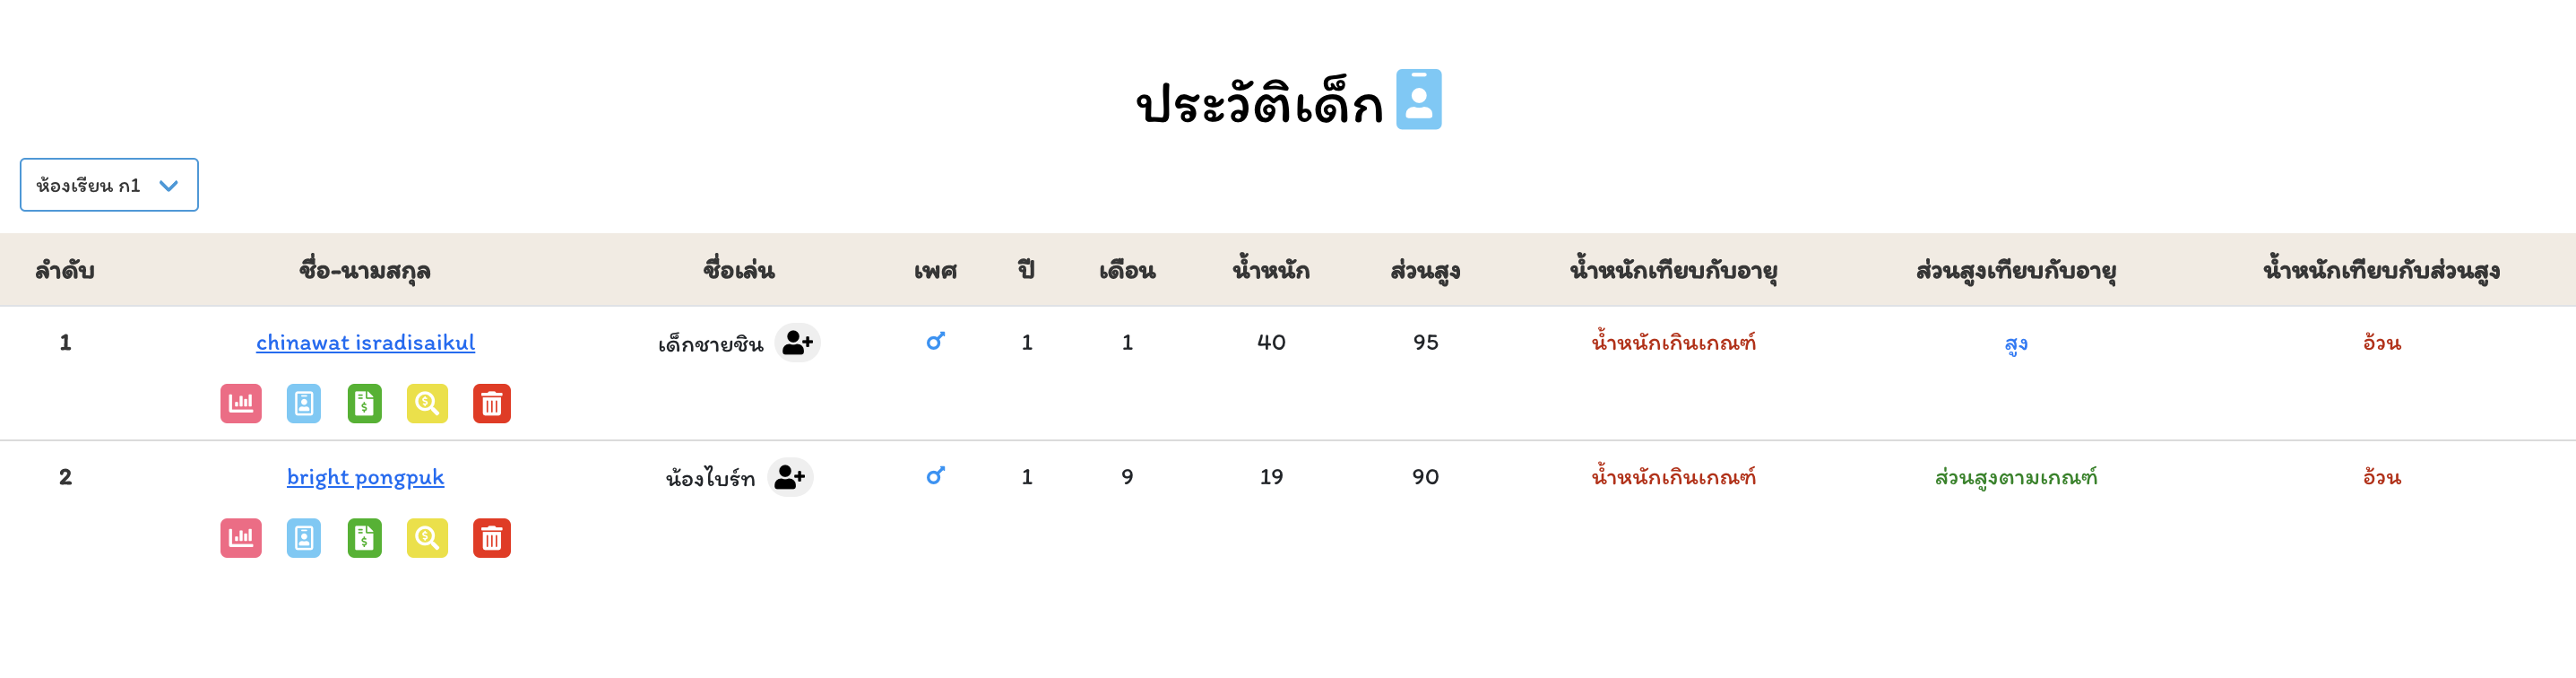
\includegraphics[width=\linewidth]{images/Profile.png}
    \end{center}
    \caption[Poem]{หน้าประวัติเก่า}
    \label{fig:ProfileNew}
\end{figure}

\begin{figure}
    \begin{center}
      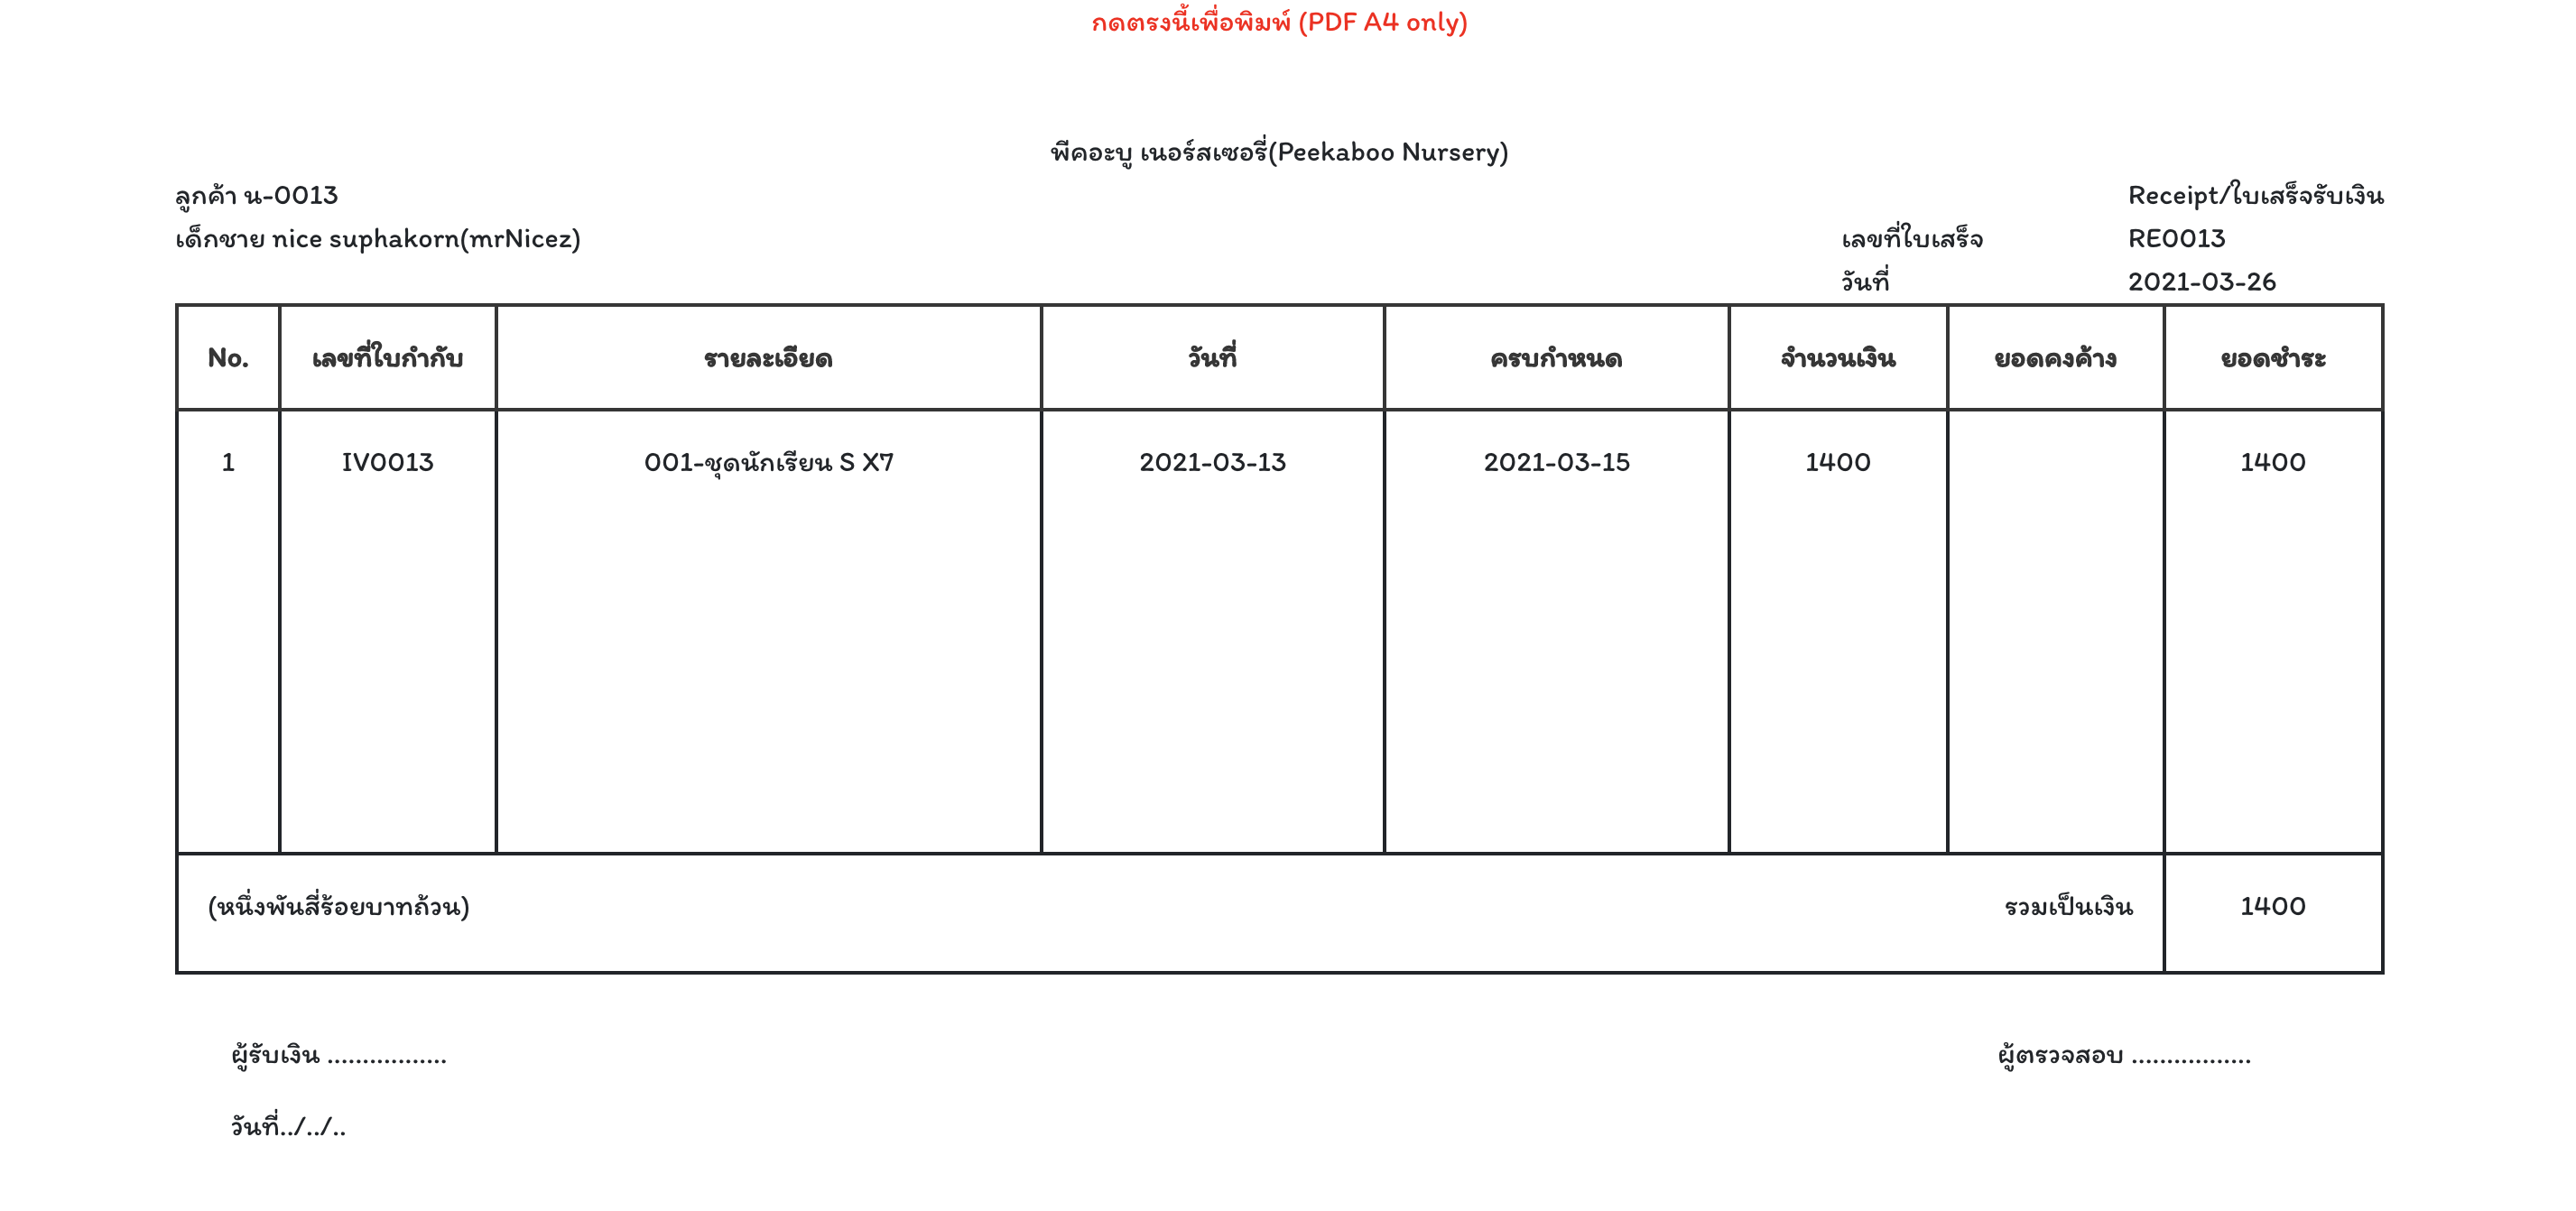
\includegraphics[width=\linewidth]{images/slipPage.png}
    \end{center}
    \caption[Poem]{ใบเสร็จ}
    \label{fig:Slip}
\end{figure}

\begin{figure}
    \begin{center}
      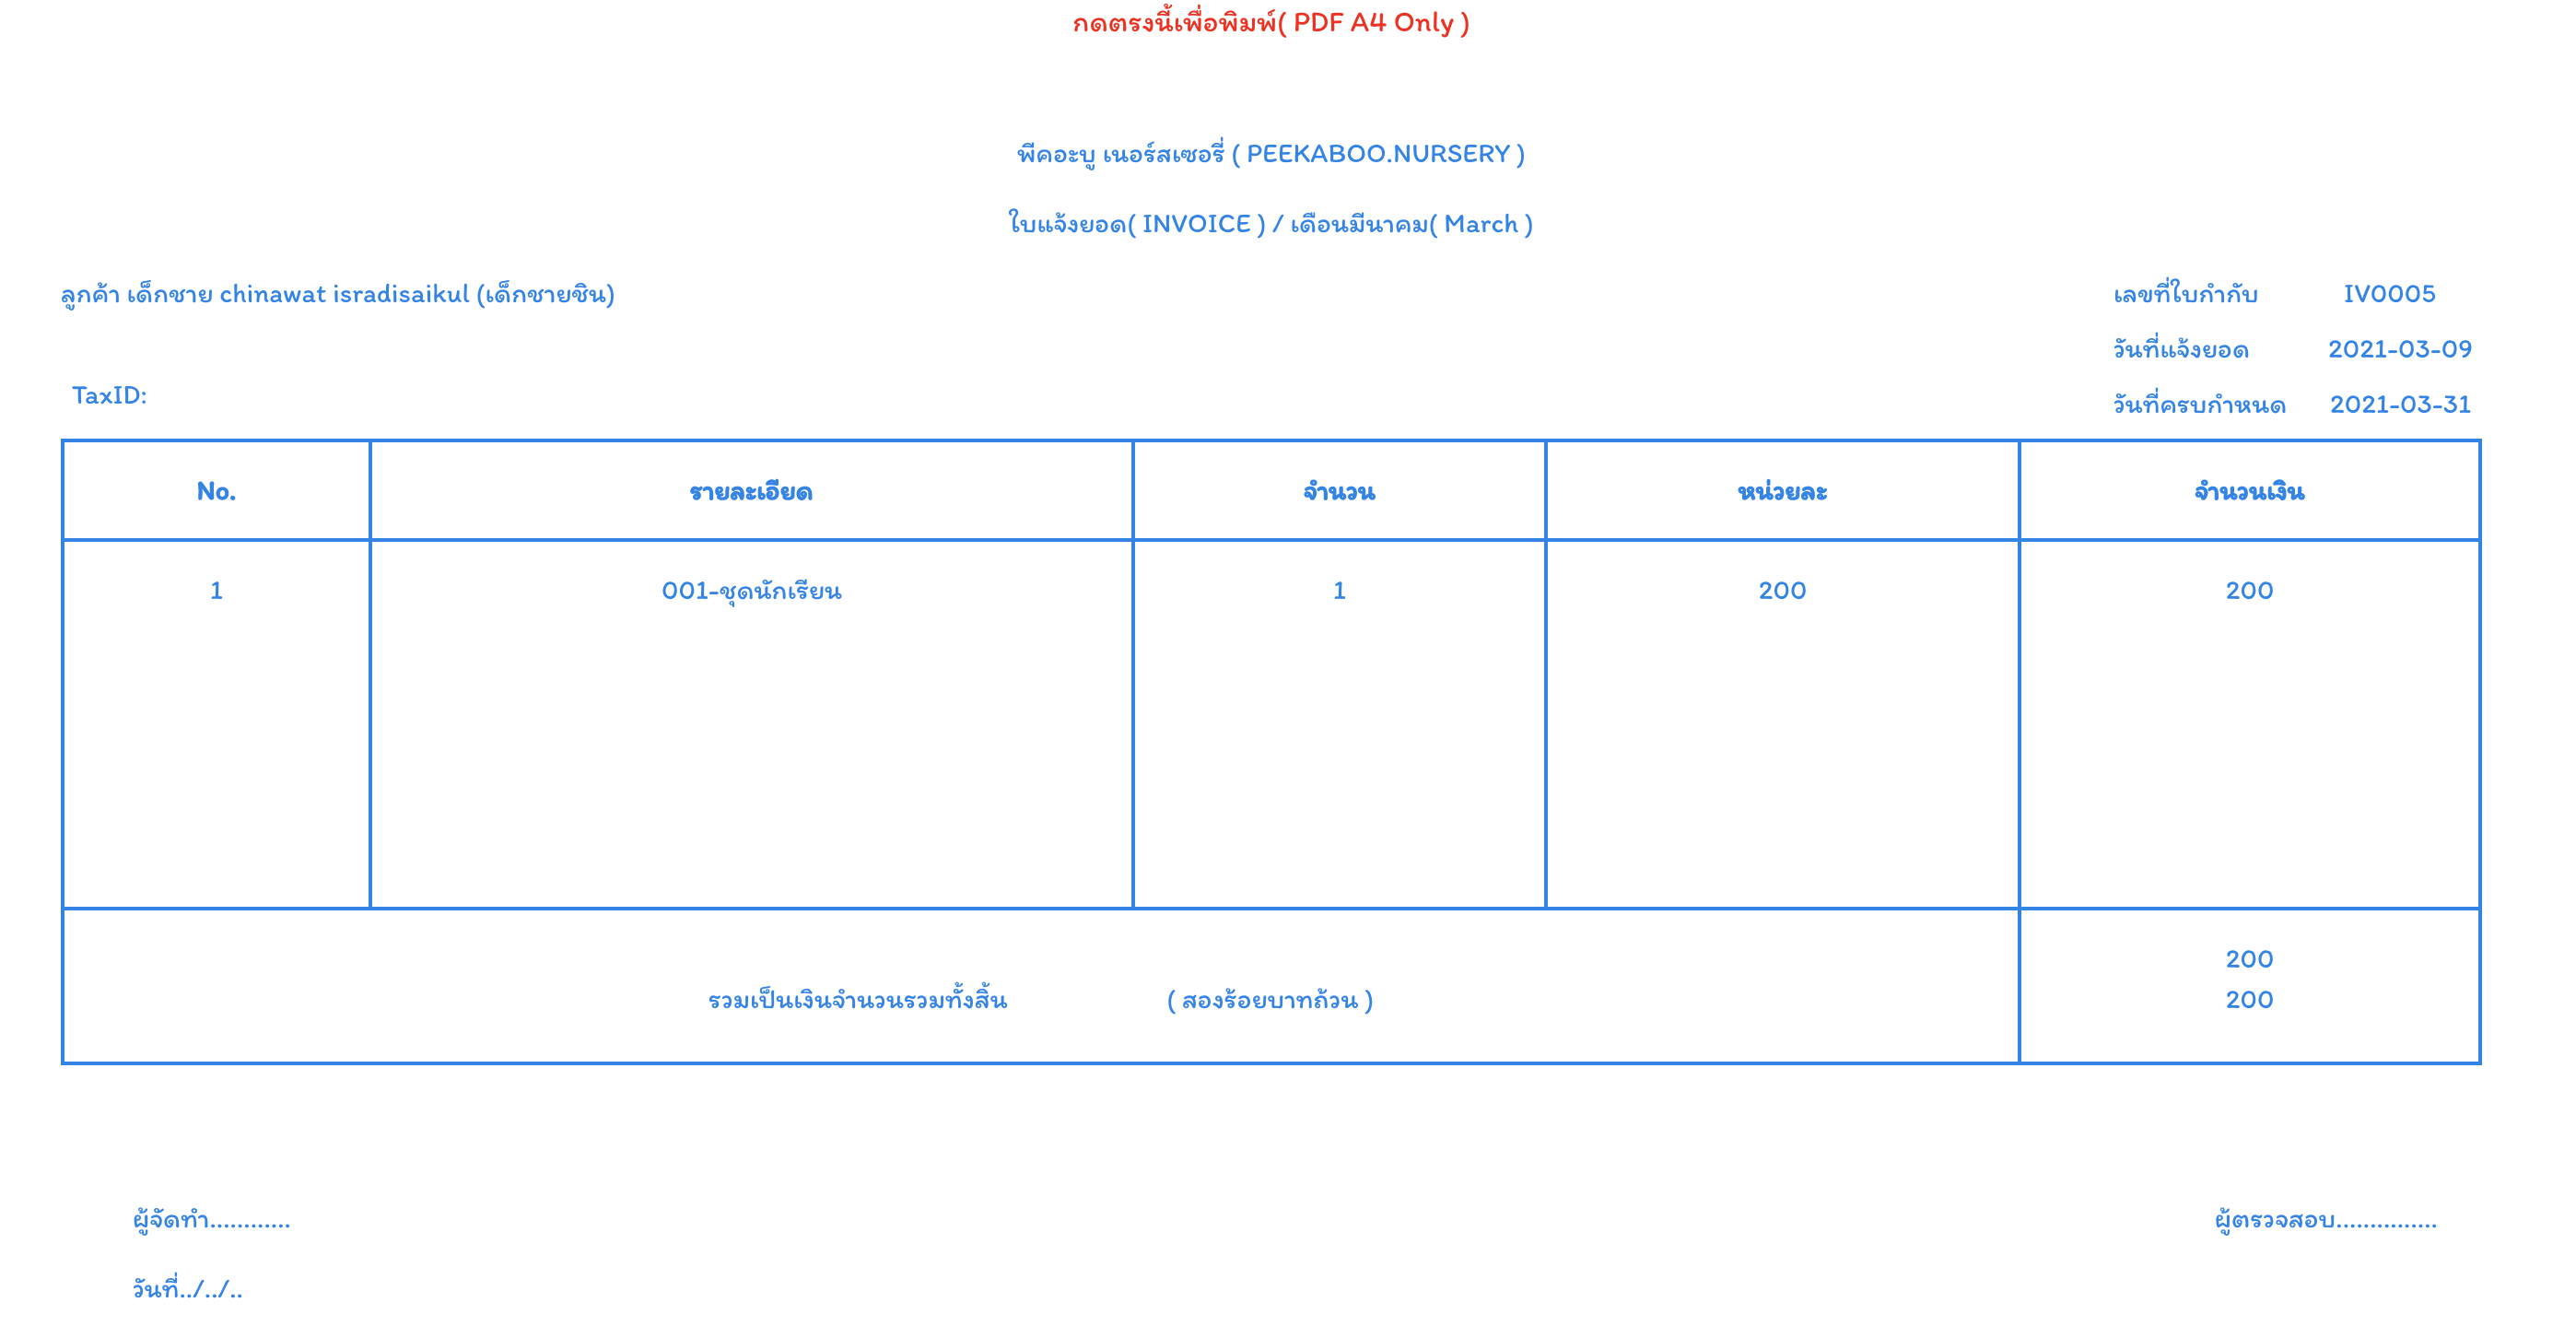
\includegraphics[width=\linewidth]{images/invoicePage.png}
    \end{center}
    \caption[Poem]{ใบแจ้งยอด}
    \label{fig:invoice}
\end{figure}

\begin{figure}
    \begin{center}
      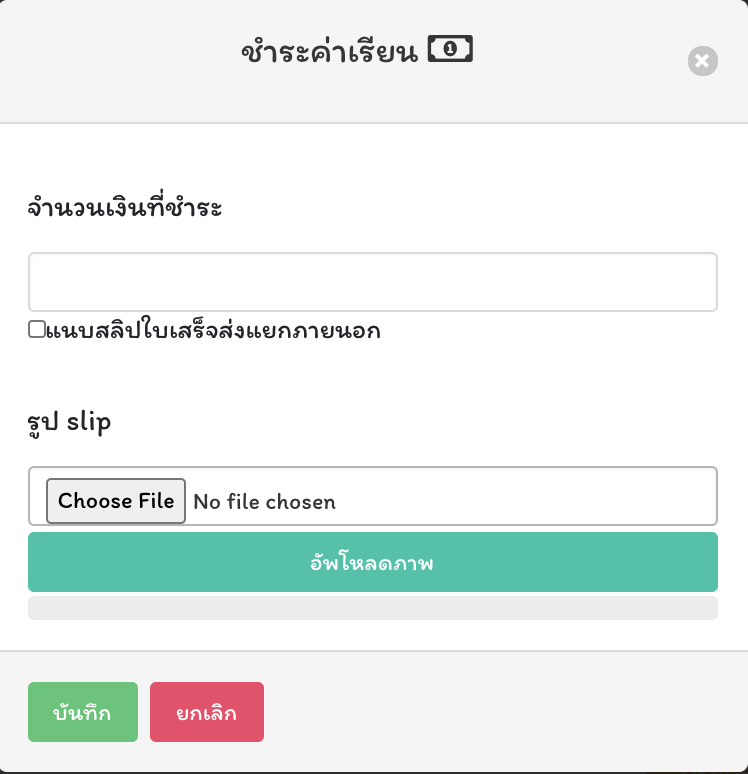
\includegraphics[width=\linewidth]{images/UpdatePayment.png}
    \end{center}
    \caption[Poem]{สามารถเลือกแนบสลิปจากภายนอกได้}
    \label{fig:UpdatePay}
\end{figure}

\begin{figure}
    \begin{center}
      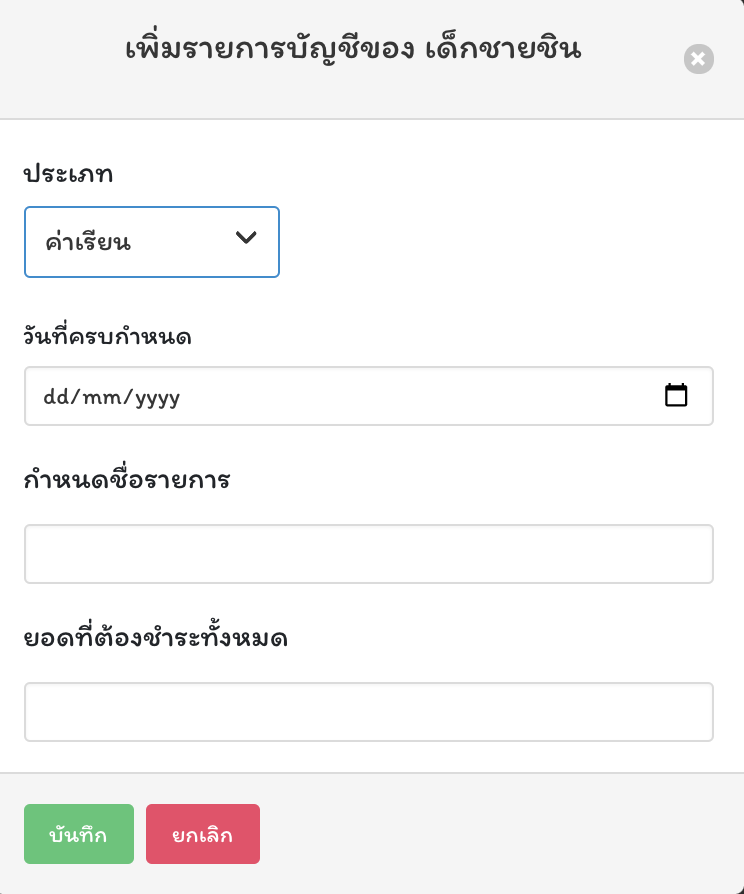
\includegraphics[width=\linewidth]{images/CreatePayment.png}
    \end{center}
    \caption[Poem]{เพิ่มรายการบัญชี}
    \label{fig:CreatePay}
\end{figure}

\begin{figure}
    \begin{center}
      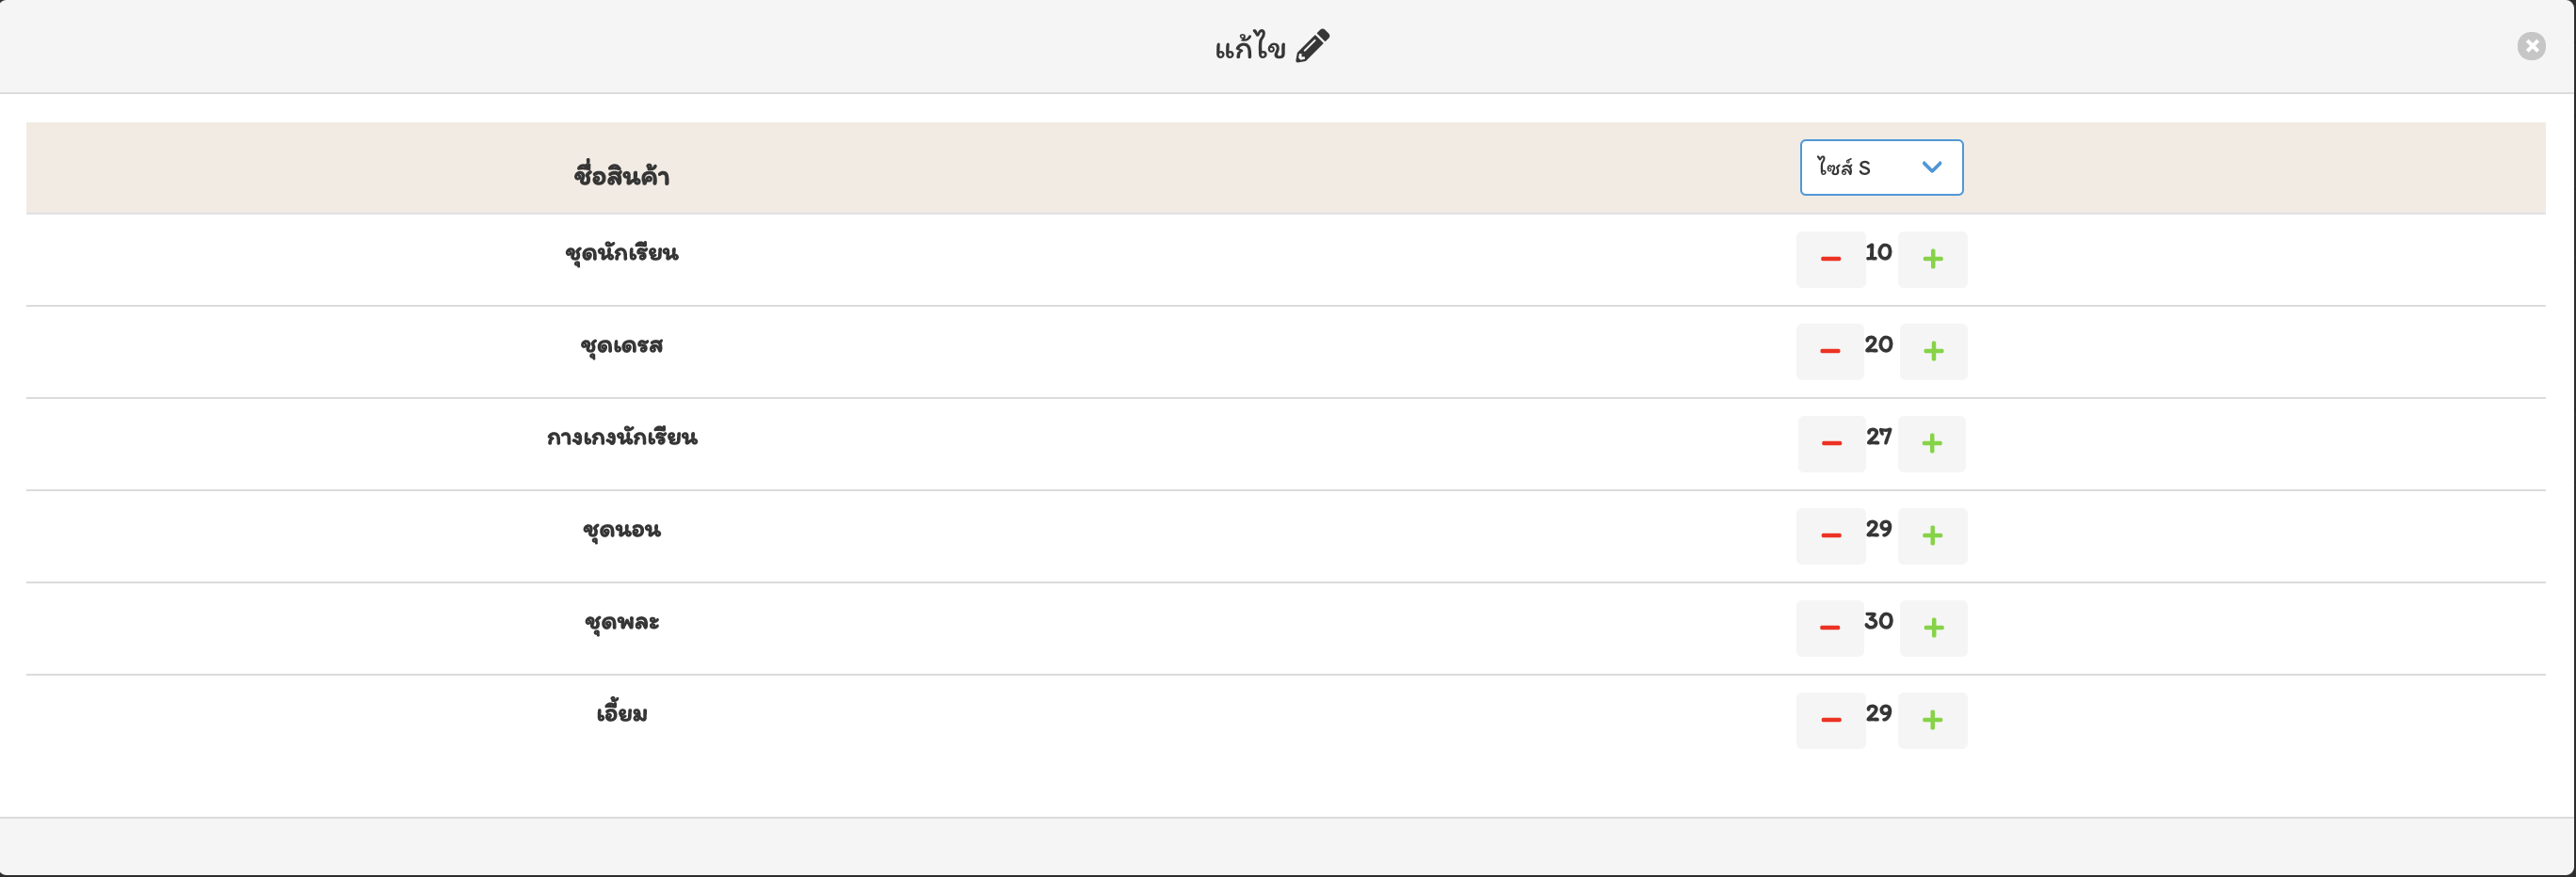
\includegraphics[width=\linewidth]{images/handleStock.png}
    \end{center}
    \caption[Poem]{แก้ไขจำนวนสินค้า}
    \label{fig:handlestock}
\end{figure}

\begin{figure}
    \begin{center}
      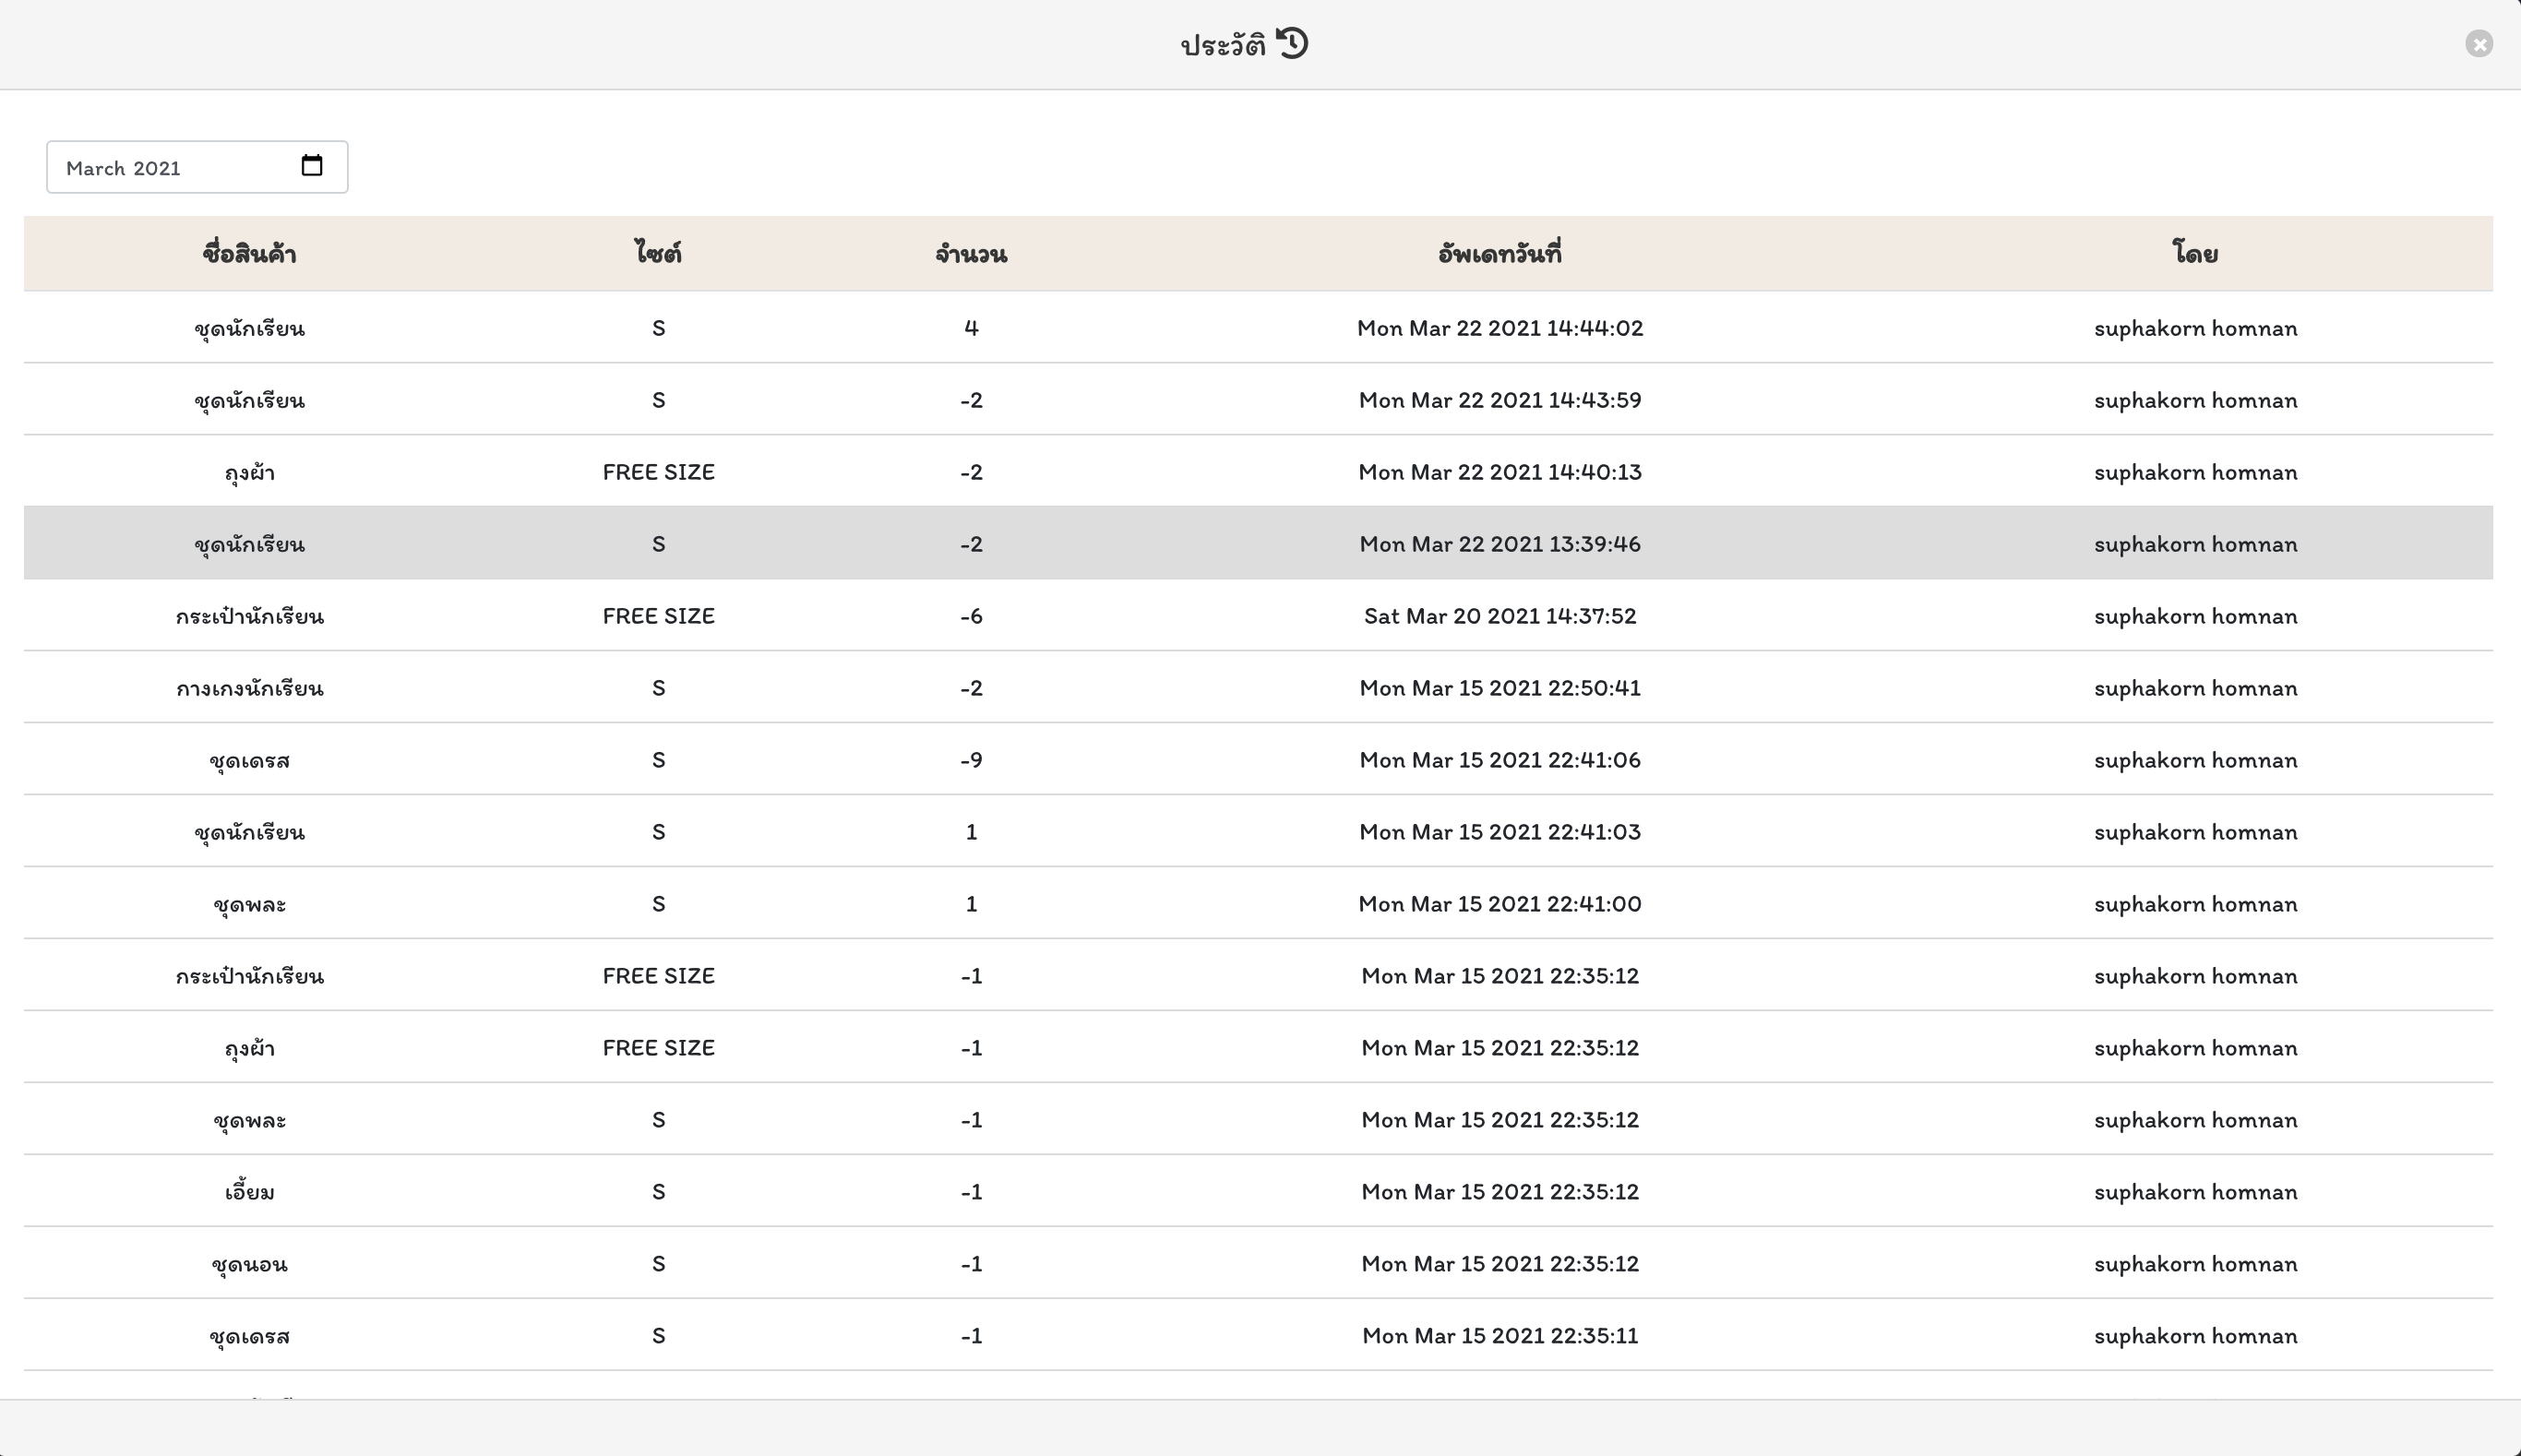
\includegraphics[width=\linewidth]{images/historyStock.png}
    \end{center}
    \caption[Poem]{ประวัติการตัดStock}
    \label{fig:historystock}
\end{figure}

\begin{figure}
    \begin{center}
      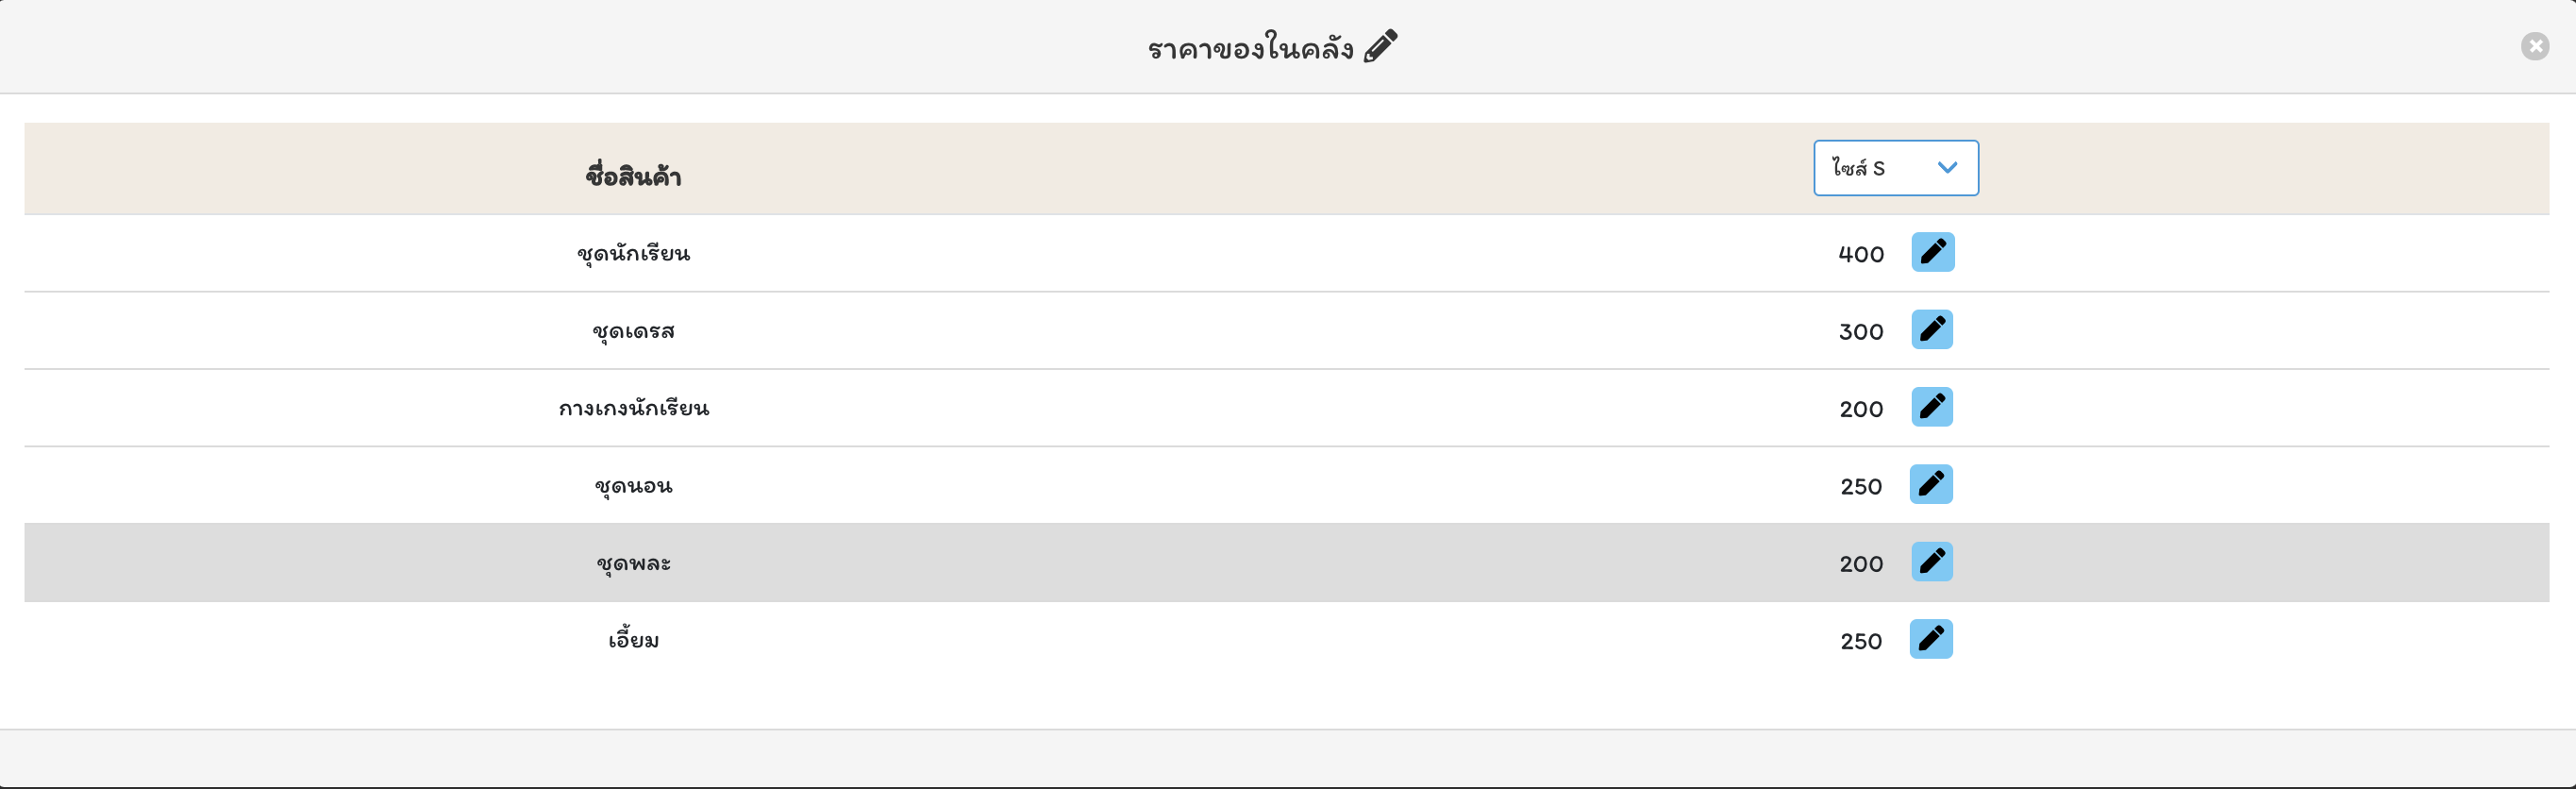
\includegraphics[width=\linewidth]{images/editPrice.png}
    \end{center}
    \caption[Poem]{แก้ราคาสินค้า}
    \label{fig:editprice}
\end{figure}


\section{Feedback จากทางาง nursery}
\paragraph{ระบบบัญชี}
\begin{itemize}
    \item ยังไม่มีใบแจ้งยอดและใบเสร็จ
    \item ใบเสร็จไม่สามารถแนบสลิปจากภายนอกได้
    \item การเพิ่มรายการบัญชีไม่สามารถเลือกประเภทของสิ่งของต่างๆได้ 
\end{itemize}
\paragraph{ระบบคลังสินค้า}
\begin{itemize}
    \item ราคาของสิ้นค้าไม่สามารถแก้ไขได้
    \item ไม่สามารถหักจำนวนของสินค้าอัตโนมัติได้
\end{itemize}

\section{แก้ไขตาม Feedback}
\paragraph{ระบบบัญชี}
\begin{itemize}
    \item ออกแบบให้ใช้งานได้ง่ายมากยิ่งขึ้น (รูปที่~\ref{fig:PaymentNew})
    \item เพิ่มใบเสร็จและใบแจ้งยอด (รูปที่~\ref{fig:Slip}, \ref{fig:invoice})
    \item ใบเสร็จสามารถแนบสลิปจากภายนอกได้ (รูปที่~\ref{fig:UpdatePay})
    \item การเพิ่มรายการบัญชีสามารถเลือกประเภทของสิ่งของต่างๆได้ (รูปที่~\ref{fig:CreatePay})
\end{itemize}
\paragraph{ระบบคลังสิ้นค้า}
\begin{itemize}
    \item ออกแบบให้ใช้งานได้ง่ายมากยิ่งขึ้น (รูปที่~\ref{fig:StockNew})
    \item ราคาของสินค้าสามารถแก้ไขได้ (รูปที่~\ref{fig:editprice})
    \item สามารถหักจำนวนของสินค้าอัตโนมัติได้ (รูปที่~\ref{fig:handlestock}, \ref{fig:historystock})
\end{itemize}
\paragraph{หน้าประวัติ}
\begin{itemize}
    \item แก้ไขให้ใช้งานง่ายมากยิ่งขึ้น (รูปที่~\ref{fig:ProfileNew})
\end{itemize}



